We apply the estimation methods to proxies of two seperate systems: The Atlantic meridional overturning circulation (AMOC), where these methods were initially used \cite{Ditlevsen2023} and global climate variations.
\subsection{Tipping of the Atlantic meridional overturning circulation}
For the AMOC the time series we consider is the sea surface temperature (SST) anomaly in the subpolar gyre in the north Atlantic ocean in comparison to the the global mean SST anomaly. The SG SST minus twice GM SST has been argued to be a proxy of the strengh of the AMOC; twice is used in compensation for the amplificaiton of global warming in the polar regions \cite[caption of figure 1]{Ditlevsen2023}.
\begin{figure}[h!]
    \begin{center}
    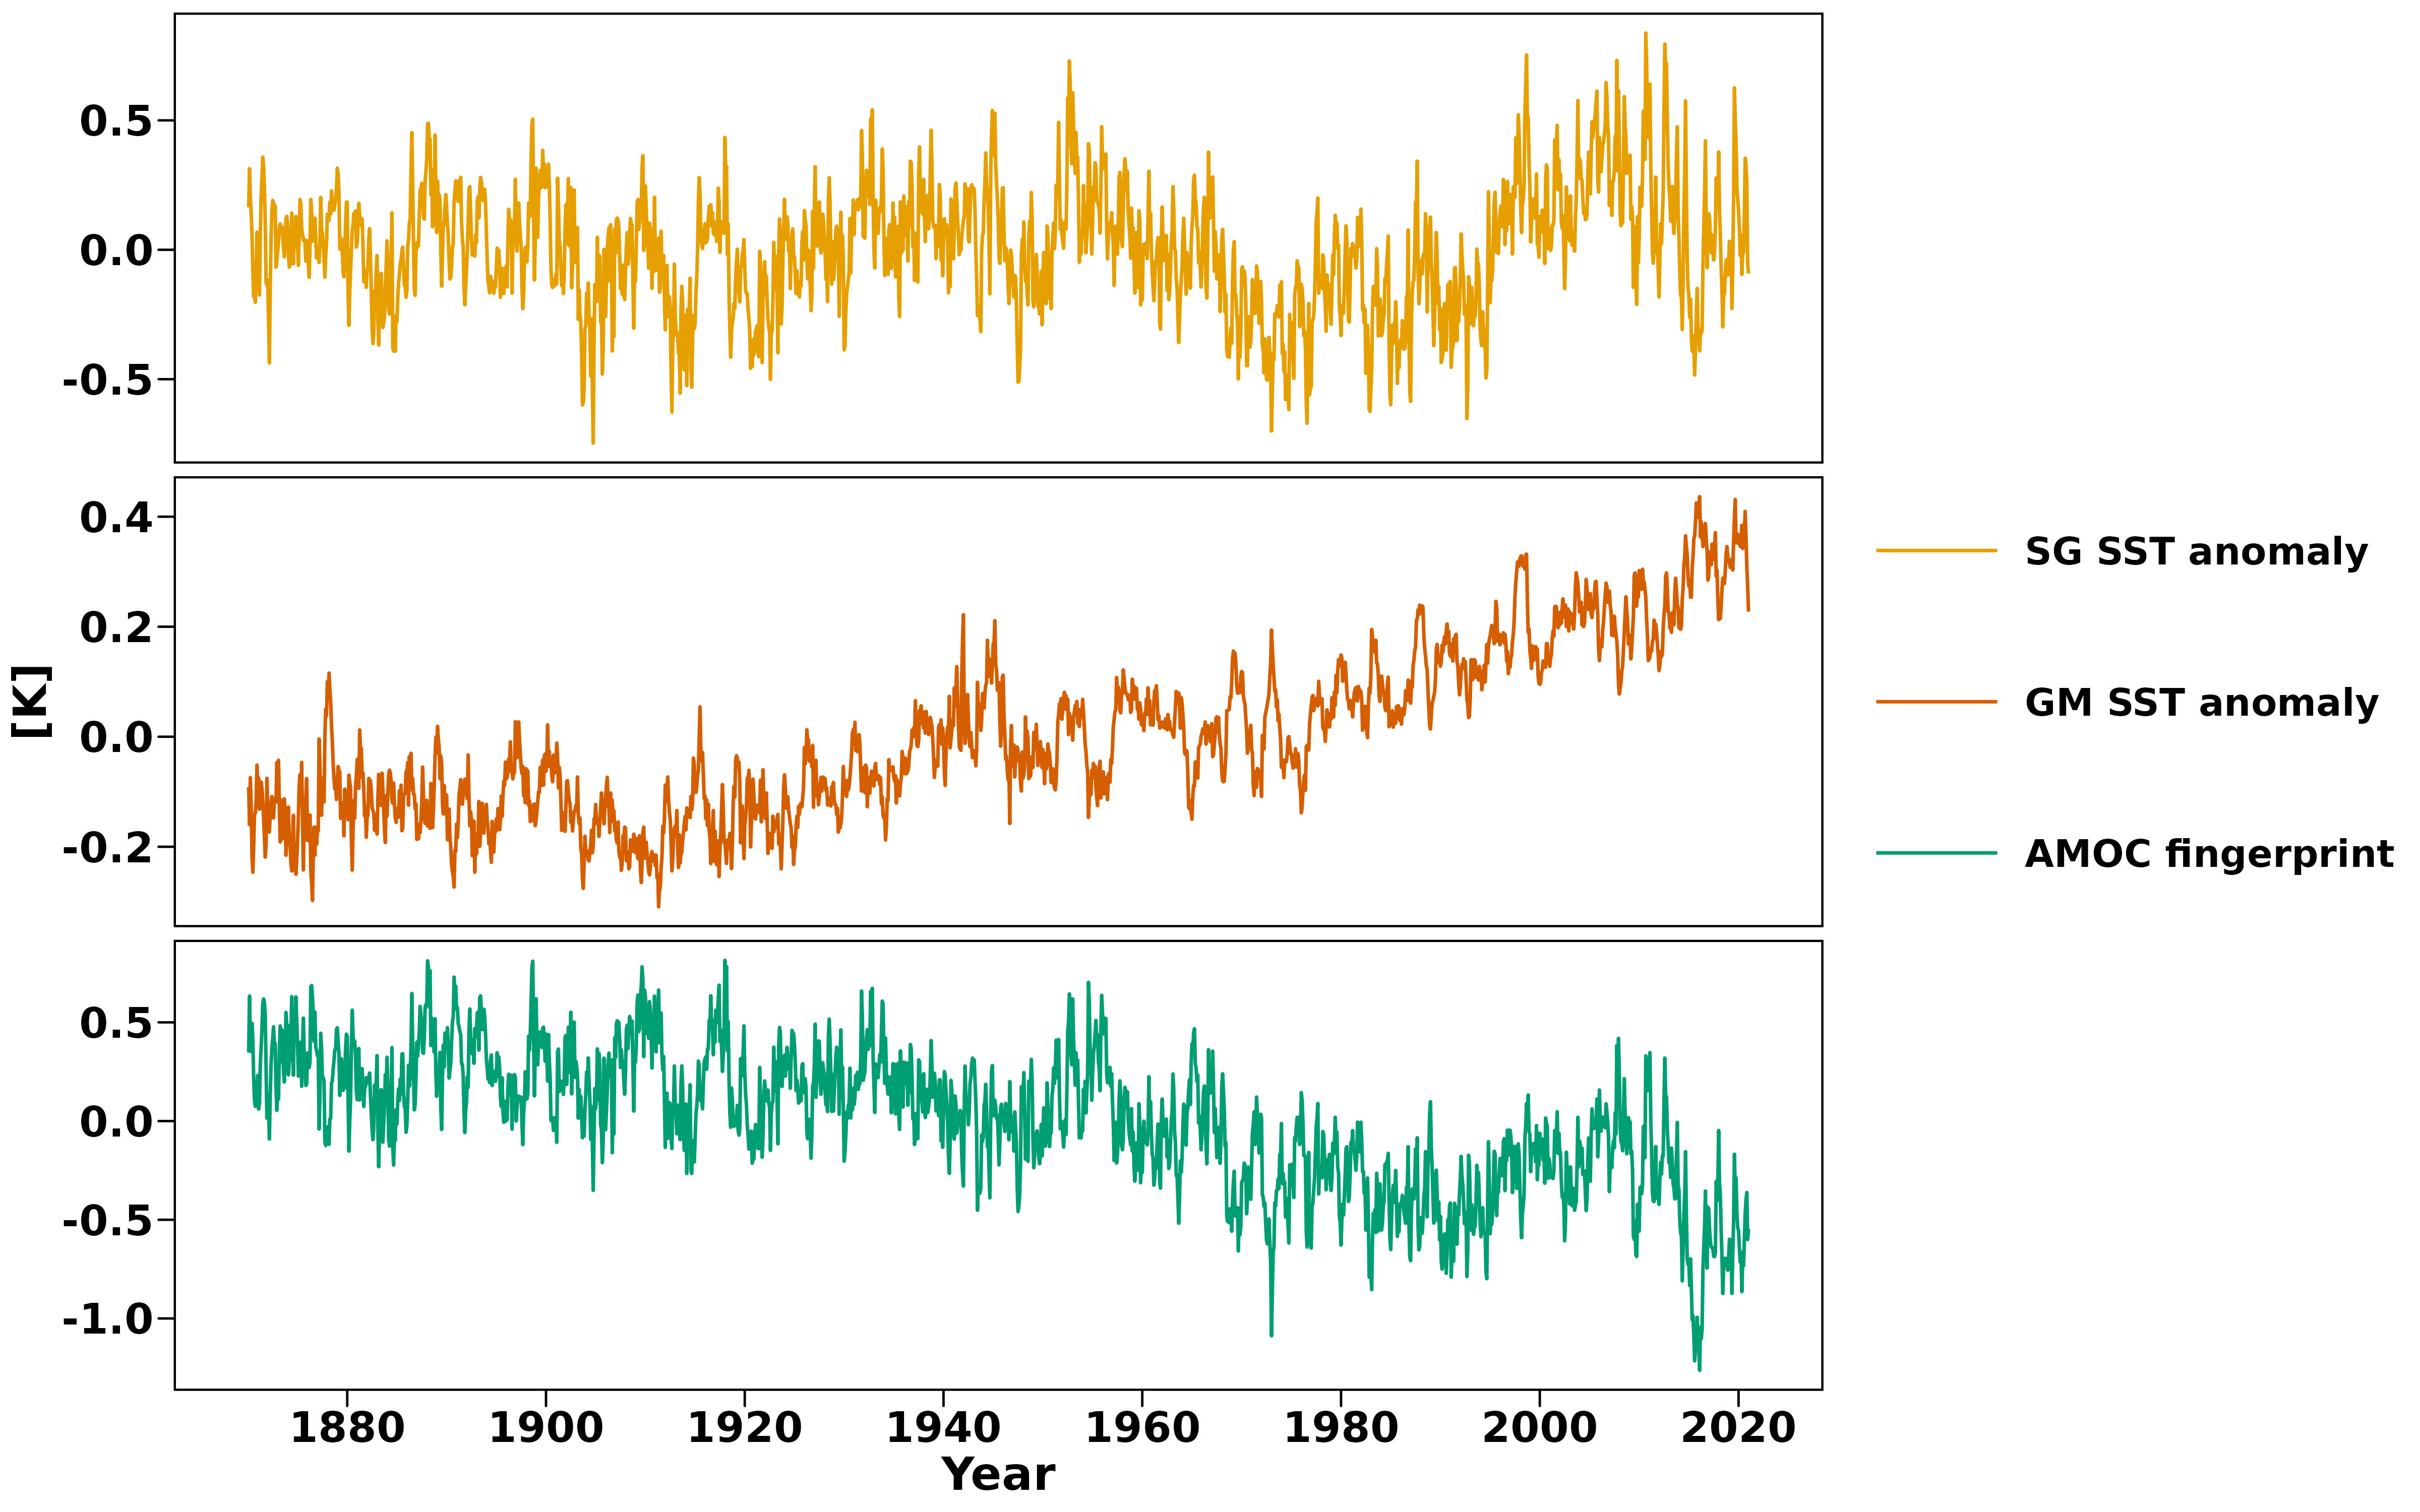
\includegraphics[scale = .075]{figures/AMOC_data_plot.jpeg}
    \caption{SST anomalies in the subpolar gyre and global mean as well as the AMOC fingerprint}
    \label{figure:AMOC_plot}
    \end{center}
\end{figure}
\subsection{Tipping in global climate variations}
Climate physicists have extensively studied ice core data from Greenland as the Greenland ice sheet acts as a sediment for the atmosphere. It is widely accepted that the ratio between the isotopes $^{18}\mathrm{O}$ and $^{16}\mathrm{O}$ is an indicator of the temperature at the time of accumulation. Additionally, $\mathrm{Ca}^{2+}$-ions from dust settle in the ice layer by layer. Unlike the ratio they do not diffuse as much; this allows us to have a finer temporal resolution. We can use calcium-ions instead of the ratio, because there is a negative correlation betwen the logarithm of the log-concetration of the $\mathrm{Ca}^{2+}$-ions and the isotope-ratio. This means that higher calcium-ion concentrations indicate colder global conditions. The ice-core data consists of observations of the oxygen isotope ratio and $\mathrm{Ca}^{2+}$-ion concentrations from $107620$ years before present to $10260$ years before present with a constant temporal resolution of $20$ years. We rescale to kilo years and focus on the observation of the calcium-ion between $86$ kilo years before present (kyrs bp) and $55$ kyrs bp; of course still with $\Delta t = 0.02$. Now, transforming ion-concentrations by $-\log (x)$ is a common practice in chemistry, whence we also consider $-\log([\mathrm{Ca}^{2+}]) - C$, where $C$ is a constant that makes the process have mean zero. We depict the ion-concetration over time
\begin{figure}[h!]
    \begin{center}
    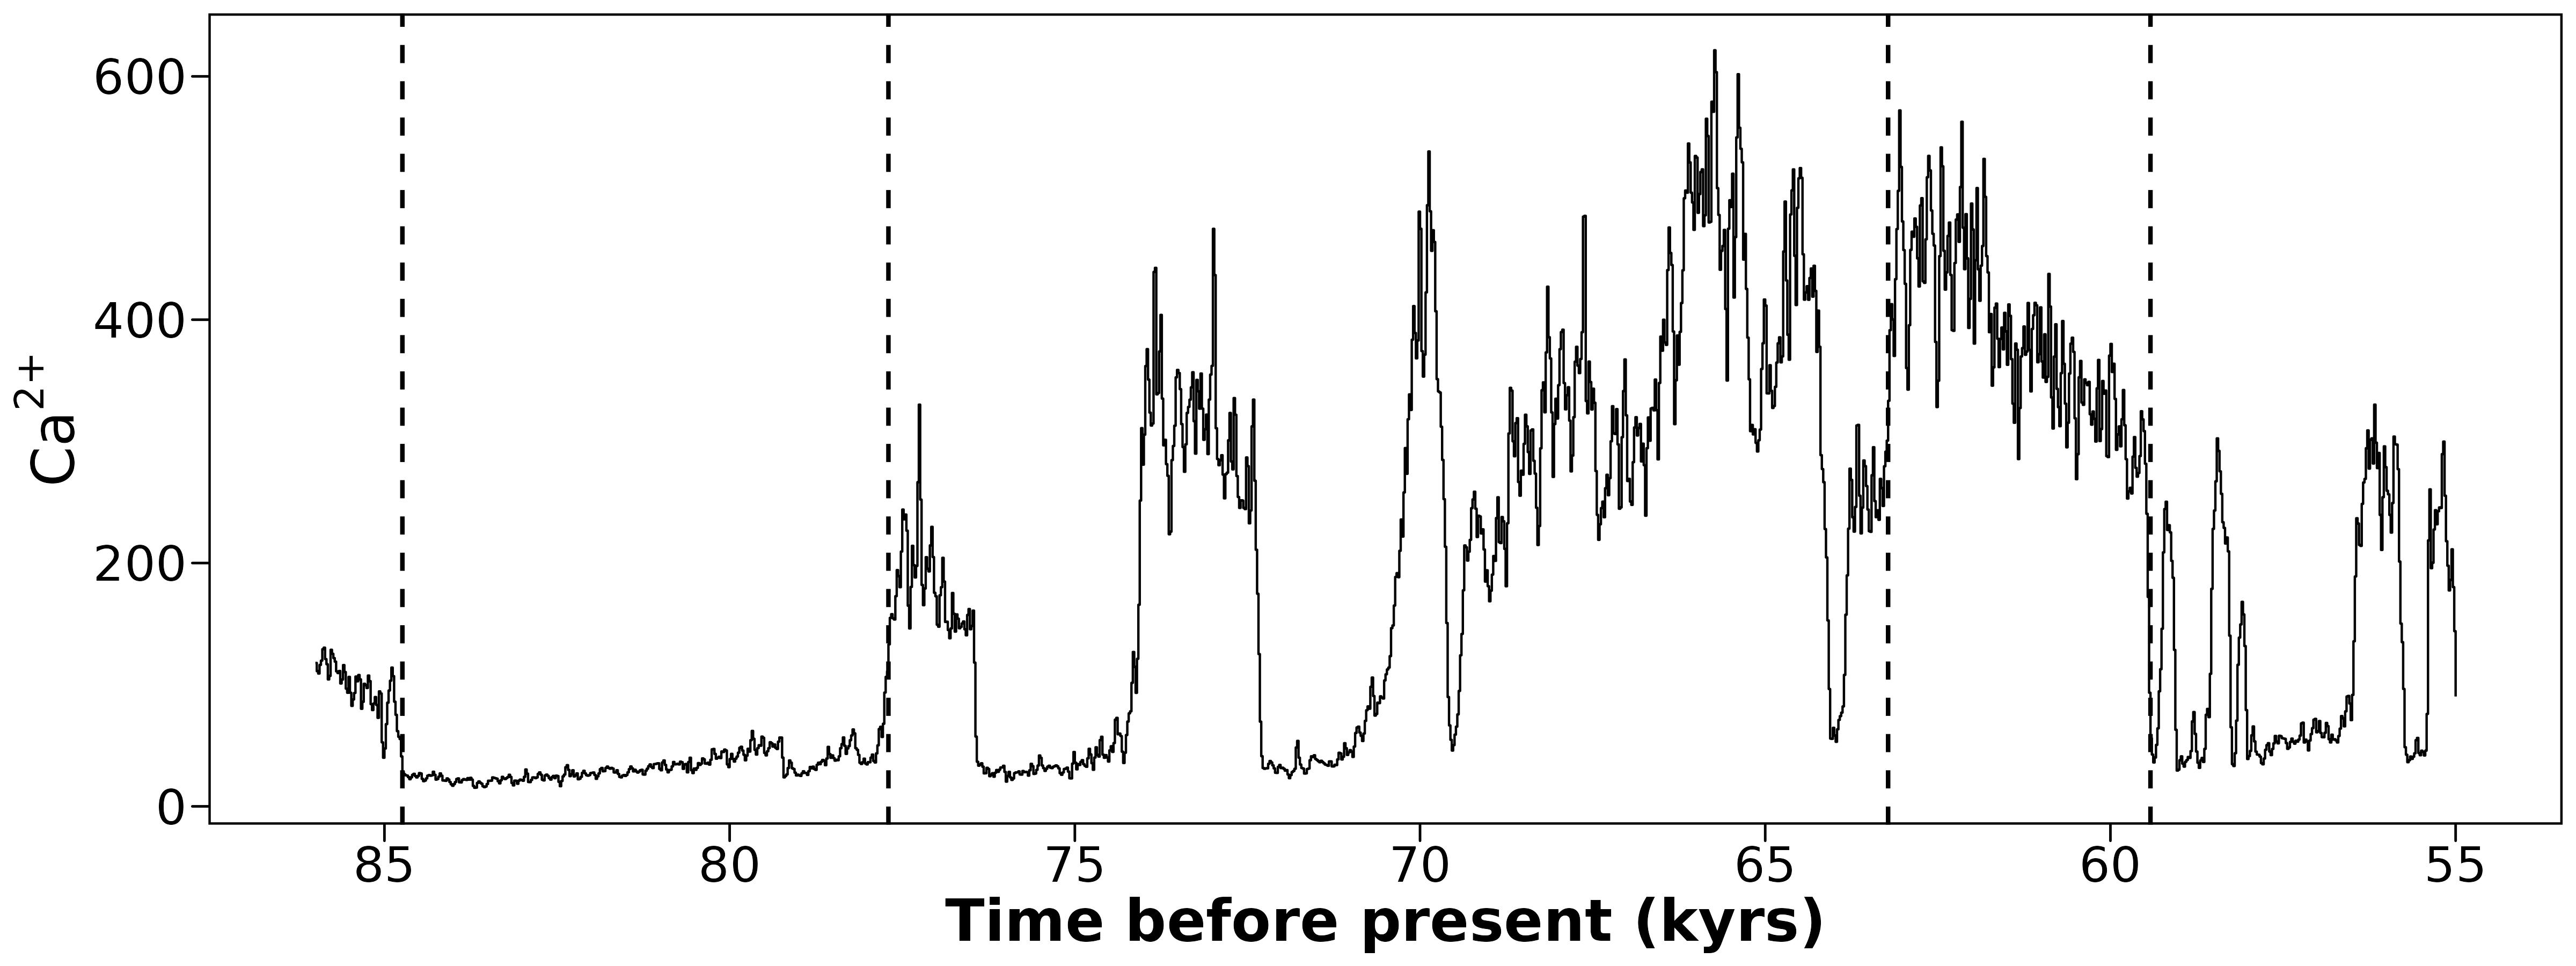
\includegraphics[scale = .075]{figures/ice_core_plot.jpeg}
    \caption{$\mathrm{Ca}^{2+}$-concetration in the ice sheet in the periode 86 kyrs bp to 55 kyrs bp}
    \label{figure:Ca_icesheet}
    \end{center}
\end{figure}\\
Looking at graph there are some periods of time where the concetration seem to be in somewhat of a stationary state. We have marked two periods that highlights to such periods by four vertical lines. The two periods we consider concentrations for are $[77.7, 84.74]$ and $[59.42, 63.22]$; these consist of 353 and 191 observations respectively. At the end of the two periods there seem to be a tipping to another state; to make this clear we zoom in on the time periods - note that we add some of the observations after tipping for illustrative purposes
\begin{figure}[h!]
    \begin{center}
    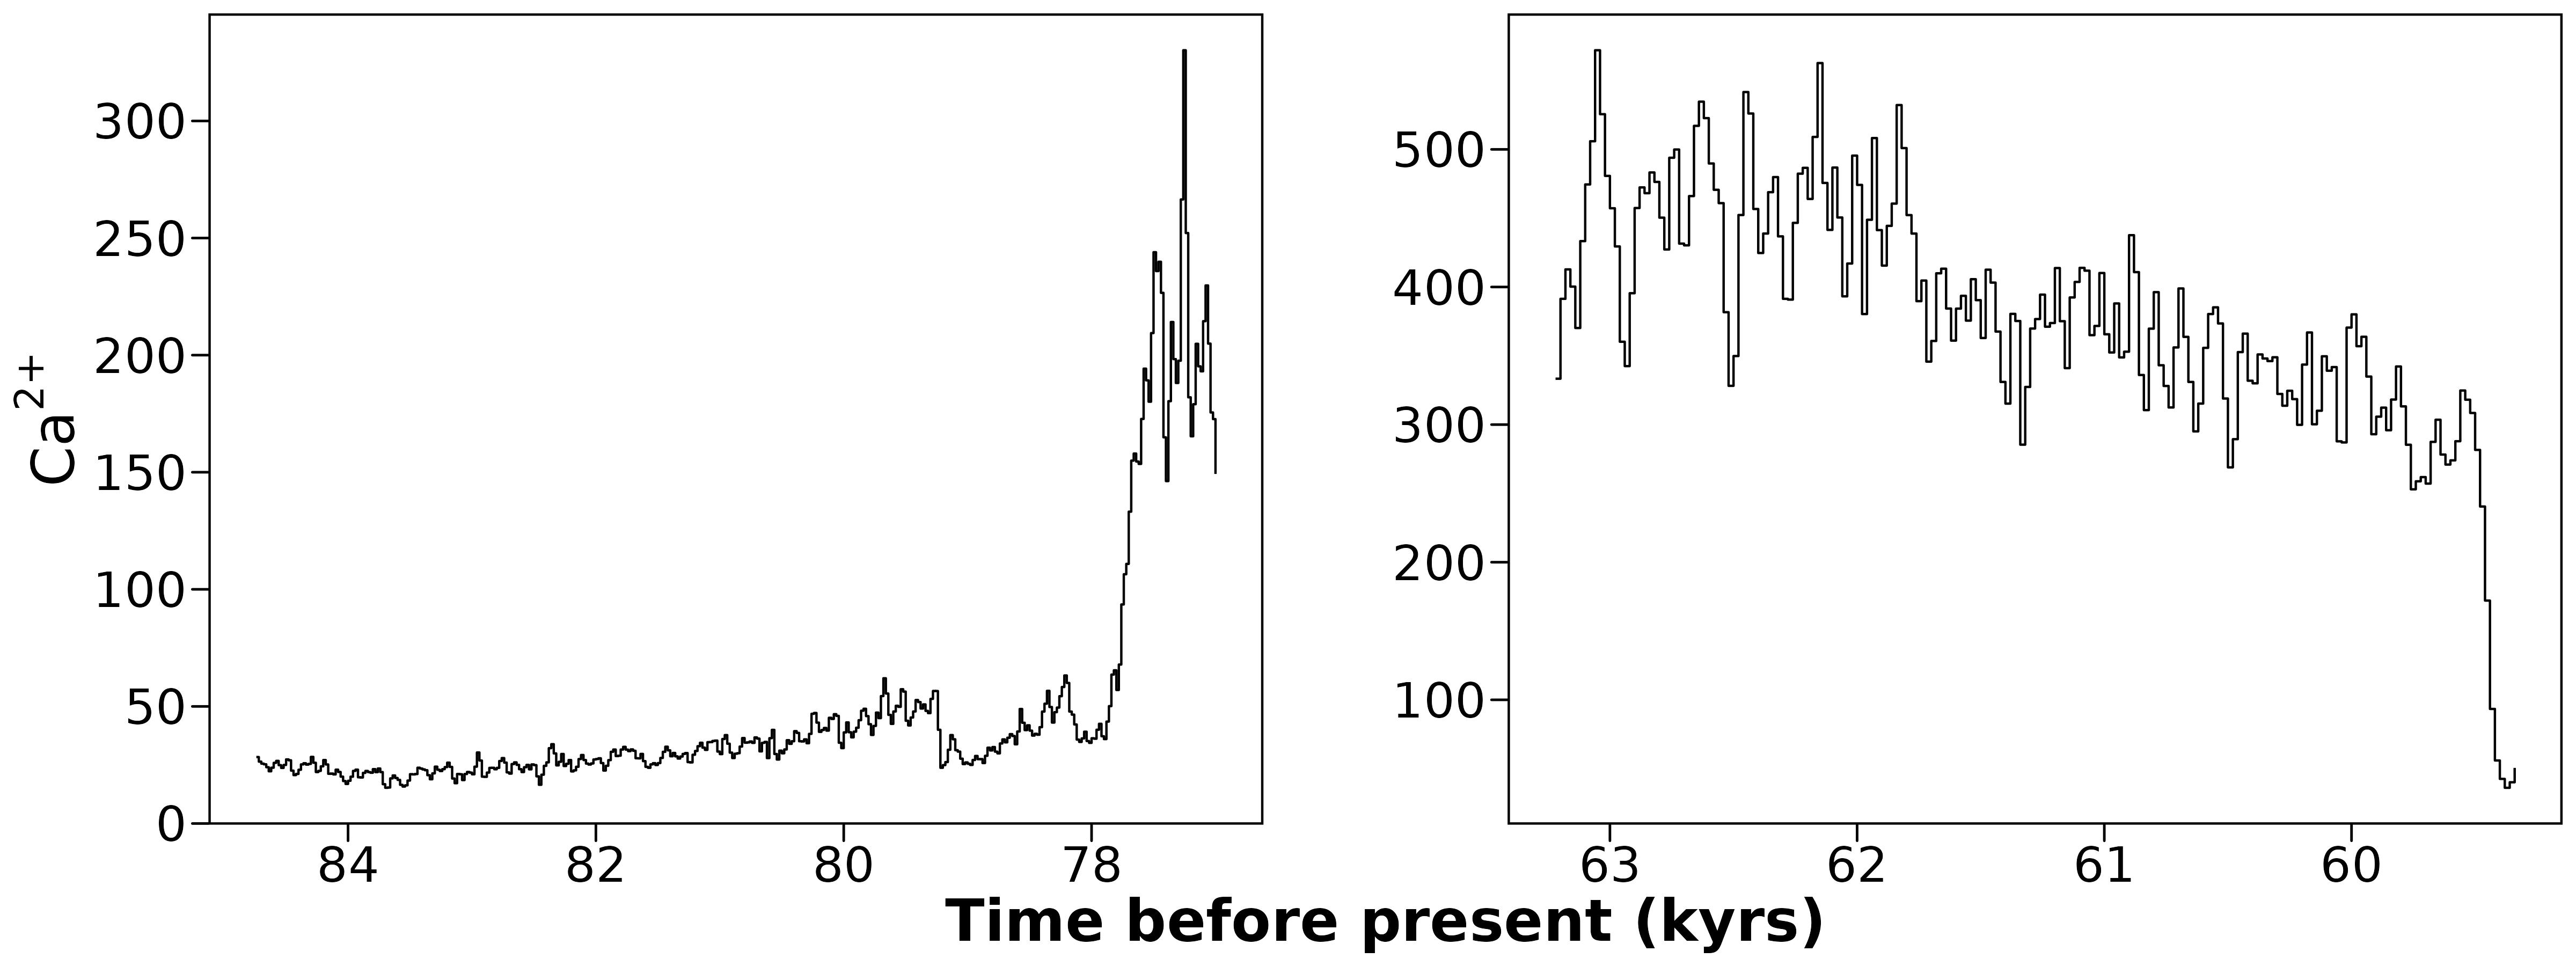
\includegraphics[scale = .075]{figures/ice_core_zoom_plot.jpeg}
    \caption{Zoom in on the $\mathrm{Ca}^{2+}$-concetration in the ice sheet in the two intervals of interest}
    \label{figure:Ca_icesheet}
    \end{center}
\end{figure}\\
We analyze both these periods using the mean-reverting geometric brownian motion based model.